\documentclass[11pt,a4paper]{article}

\usepackage{url,,}
\usepackage{graphicx}
\usepackage{hyperref}
\usepackage{amsfonts}
\usepackage{amssymb}
\usepackage{amsmath}
\usepackage{multirow}
\usepackage{listings}
\usepackage{fullpage}
\usepackage{fancyhdr,a4wide}
\usepackage{makeidx}
\usepackage{placeins}
%\usepackage[procnames,noindent]{lgrind}

\lstset{ %
language=VHDL,                % choose the language of the code
basicstyle=\footnotesize,       % the size of the fonts that are used for the code
showstringspaces=false,         % underline spaces within strings
%numbers=left,                   % where to put the line-numbers
%numberstyle=\footnotesize,      % the size of the fonts that are used for the line-numbers
%stepnumber=1,                   % the step between two line-numbers. If it's 1 each line will be numbered
%numbersep=5pt,                  % how far the line-numbers are from the code
%backgroundcolor=\color{white},  % choose the background color. You must add \usepackage{color}
showspaces=false,               % show spaces within strings adding particular underscores
showtabs=false,                 % show tabs within strings adding particular underscores
escapeinside={\%*}{*)}          % if you want to add a comment within your code
}

\begin{document}	

\begin{titlepage}

\thispagestyle{fancy}
\lhead{}
\chead{
\large{\textit{
Informatics and Mathematical Modelling\\
Technical University of Denmark}}}
\rhead{}
\rule{0pt}{50pt}
\vspace{3cm}

\begin{center}
 	\huge{\textbf{02207 : Advanced Digital Design Techniques}}\\
 	\vspace{1cm}
 	\huge{Low-pass Filter (2 x 1-D)}\\
 	\vspace{1cm}
 	\huge{\textit{Examination Project}}\\
 	\vspace{1cm}
 	\huge{Group \textit{dt07}}\\
\end{center}

\vspace{4cm}

\begin{flushright}
	\LARGE{Markku Eerola (s053739)}\\
	\vspace{0.3cm}
	\LARGE{Rajesh Bachani (s061332)}\\
	\vspace{0.3cm}
	\LARGE{Josep Renard (s071158)}\\
\end{flushright}
\cfoot{\today}
\end{titlepage}

\newpage 
\tableofcontents

\newpage

\section{Introduction}
The project that we have implemented is a 2x1D filter of size 3x3 for convolution of an image of size 256x256 pixels.  

\section{Design Architecture}
%give the block design here. we need the following figure:
%a complete diagram of the processor - indicating the input and output signals, and also containing the internal blocks like the cache register,filter register, fsm_in, the multipliers, adders, mux, and fsm_out.
The overall design of the filter unit can be seen in figure \ref{fig:proc}. More detailed architecture can be seen in figure \ref{fig:procdetail}.

\begin{figure}[h]
	\centering
		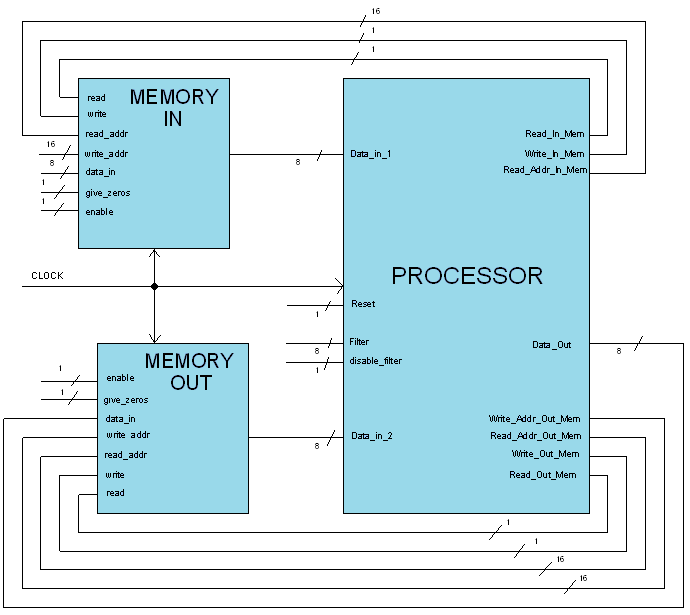
\includegraphics[width=4in]{./processador.PNG}
	\caption{Filter unit design}	\label{fig:proc}
\end{figure}

\begin{figure}[h]
	\centering
		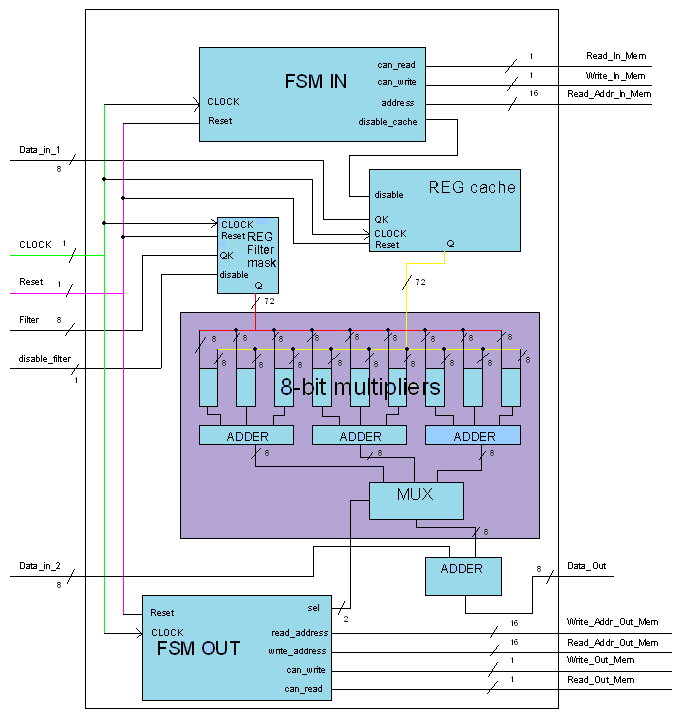
\includegraphics[width=4in]{./insideproc.PNG}
	\caption{Processor architecture}	\label{fig:procdetail}
\end{figure}
%here we should mention the details about the data path, bit widths etc. 
%we should give a brief explanation of each of the components in the architecture - just a couple of lines explanation should be good enough. 
%also we should explain the purpose of each of the input and output signals of the memory and the processor.

\FlowBarrier
\section{Sequencing of Operations}
%explain the entire sequence in which the image is convoluted. in particular
\subsection{Memory Initialization}
%how the initialization is done - the input FSM keeps the write of the input memory till 65526 clock cycles - so all the pixels are read from the hex file.
%in the meantime, the output FSM keeps the write signal of the output memory to 1 and it is initialized with 0.
In our case we have an image on format .hex, is the values of the image on hexadecimal, 2 values of 4 bits, 8 bits total, and we have to pass all the image to the memory so there are 65536 values on our image, so the processor are going to spend this amount on clock cycles, but we need too another memory to store the new values of the convolution for the next vertical filter pass. For this task we have a final state machine that is in charge to create an address and store the value on the memory with this address. So now we have to create two memories, the first one that we call memory in are going to be the values of the image to filter with their correspondent address, the final state machine generate the address and give to the memory the value of the image with their correspondent address, at the same time because are different state machine and memory, the space for the filtered image is created in a parallel way, but now the difference between the first one is that we want the memory empty, all with zeros, and we use the processor to make this operation, the final state machine for the output create the addresses and has the property to say the multiplexor of the final output which one wants, and one of the outputs is all zeros, so with that the processor knows that in this time period for initializing the memory out throws by Data\_out a value 0 all the time.
When the 65536 clock cycles are ended the memory in is with the values of the image and the memory out empty, all with values zeros.	

\subsection{Memory Read and Write by Processor}
%Once the initialization is done, 
% 1. the input fsm reads 3 pixels - and then waits for 9 clock cycles
% 2. the output fsm starts when the input fsm becomes idle - and runs the sequence read-idle-write 3 times.
%give picture from modelsim here showing how the two fsms synchronize.
When the memory in and out are initialized, is time to the processor to make the operations, but how do the processor access to the memory for read and write?, very easy, we start with the premise that the final state machine out needs to read the values of the memory out, add the new value calculated and store it on the memory, this operation costs 3 clock period, but we have 3 values each convolution so the final state machine out needs 9 clock cycles for finish all his work. Now we have to synchronize the output with the input, so the final state machine in that read 3 values on 3 clock cycles has to wait 9 clock cycles for the next read for memory, and this all the time because he may allow the output to make their own calculations. So the input data is red on periods of 3 clock cycles and wait 9 for allow the output to generate the new value and don't overwrite some value that can be modify the output.

\subsection{Memory Access Sequence}
%mention the sequence of the memory access from the input fsm and the output fsm
For the memory sequence we use a particular way, we want to access to the memory the less time possible, so we have created one kind of memory cache inside the processor, the cache consist in one ShiftRegister for store 9 pixels, the number of pixels that we need to filter with our mask of 3x3, and on the beginning the final state machine take from the memory 9 values, for fill all the cache, but on the next clock cycle only take 3 values from the memory, the next column if we are on the horizontal pass (Figure 1(file horizontal pass)) or the next row if we are on the vertical pass (Figure 2(file vertical pass)) as we can see. But the sequence has a particular thing, when the values of the memory arrives to the end of the picture now doesn't work the shiftregister because we have to come back to the beginning and start again, so when the image values seized from the memory, last column on the horizontal pass and last row on the vertical pass, there are another time 9 lectures from the memory to fill up all the shift register and continue the same mechanism like l say before.
\section{Finite State Machines}
\subsection{Input Controller}

%state machine diagram
\subsection{Output Controller}

%state machine diagram

\FlowBarrier
\section{Synthesis}
%present the results from the various reports here. 
% the critical path
% area 
% power dissipation
We synthesized the design using four different clock periods, namely 7ns, 5ns, 3ns and 2ns, and let Design Vision try to optimize the design for speed to get the fastest possible design. Turns out 2ns is the minimum clock period for our design, Design Vision was not able to synthesize a faster design even when we tried. To get meaningful power reports we simulated switching activity with the VSS Simulator and the activity was passed on to Design Vision. On top of power reports we also obtained area and timing reports from the design on all four clock cycles. The actual reports can be seen in the appendix, but a summary of the results can be seen in table \ref{tab:synth}.

\begin{table}[h]
	\caption{Summary of Design Vision reports}
	\begin{center}
		\begin{tabular}{|l|l|l|l|l|l|l|} \hline
			\textbf{T}_{C} [ns]	& \textbf{P}_{stat}	[mW] & \textbf{P}_{dyn} [mW]	& \textbf{P}_{tot} [mW] & \textbf{A}_{comb} [um^2]& \textbf{A}_{tot} [um^2] & \textbf{T}_{cp} [ns] \\ \hline
			7 & 0.11 & 1.60 & 1.71 & 44067 & 53079 & 4.7 \\ \hline
			5 & 0.11 & 1.71 & 1.82 & 44067 & 53079 & 4.7 \\ \hline
			3 & 0.13 & 2.19 & 2.32 & 49595 & 58611 & 2.9 \\ \hline
			2 & 0.20 & 2.60 & 2.80 & 58668 & 67700 & 1.9 \\ \hline
			
		\end{tabular}
	\end{center}
	\label{tab:synth}
\end{table}

\FlowBarrier
\section{Results}
%put the convoluted and the original image here to show the results.

\section{Discussion}
%explain how would the design change if the filter size is changed. parameters that would change:
%number of adders and multipliers.

\end{document}